\section{V-Modell}

\begin{tcolorbox}[title=V-Modell]
    Das \textbf{V-Modell} hilft, qualitätssichernde Maßnahmen in den Entwicklungsprozess zu integrieren.\\
    Beim Übergang der Phasen des V-Modells werden die entstandenen Modelle oder Dokumente überprüft (\textit{Review}; Phasenübergänge: \textit{Qualitätstor}), bevor mit der nächsten Phase begonnen wird.

    \begin{itemize}
        \item Nach der \textbf{Realisierung} werden einzelne Klassen oder Module im Klassen- /Modultest getestet (\textbf{Komponententest})
        \item Anschliessend \textbf{Integration} der getesteten Komponenten gemeinsame Tests, Basis; \textbf{Entwurf} (\textbf{Integrationstests}).
        \item Nach der Integration wird das gesamte System in (möglichst) realer Umgebung getestet (\textbf{Systemtest} bzw. \textbf{Werkstest}), Basis: Ergebnisse der \textbf{Analyse}.
        \item Im Anschluss wird das System  vom Kunden im \textbf{Abnahmetest} abgenommen, Basis: vertragliche Vereinbarungen, gemeinsam erarbeitete \textbf{Anforderungen}
    \end{itemize}

    \begin{itemize}
        \item \textbf{Verifikation}: Wird ein \textbf{korrektes Produkt} entwickelt?
        \item \textbf{Validierung}: Wird das \textbf{richtige Produkt} entwickelt?
    \end{itemize}


\end{tcolorbox}

\begin{figure}
    \centering
    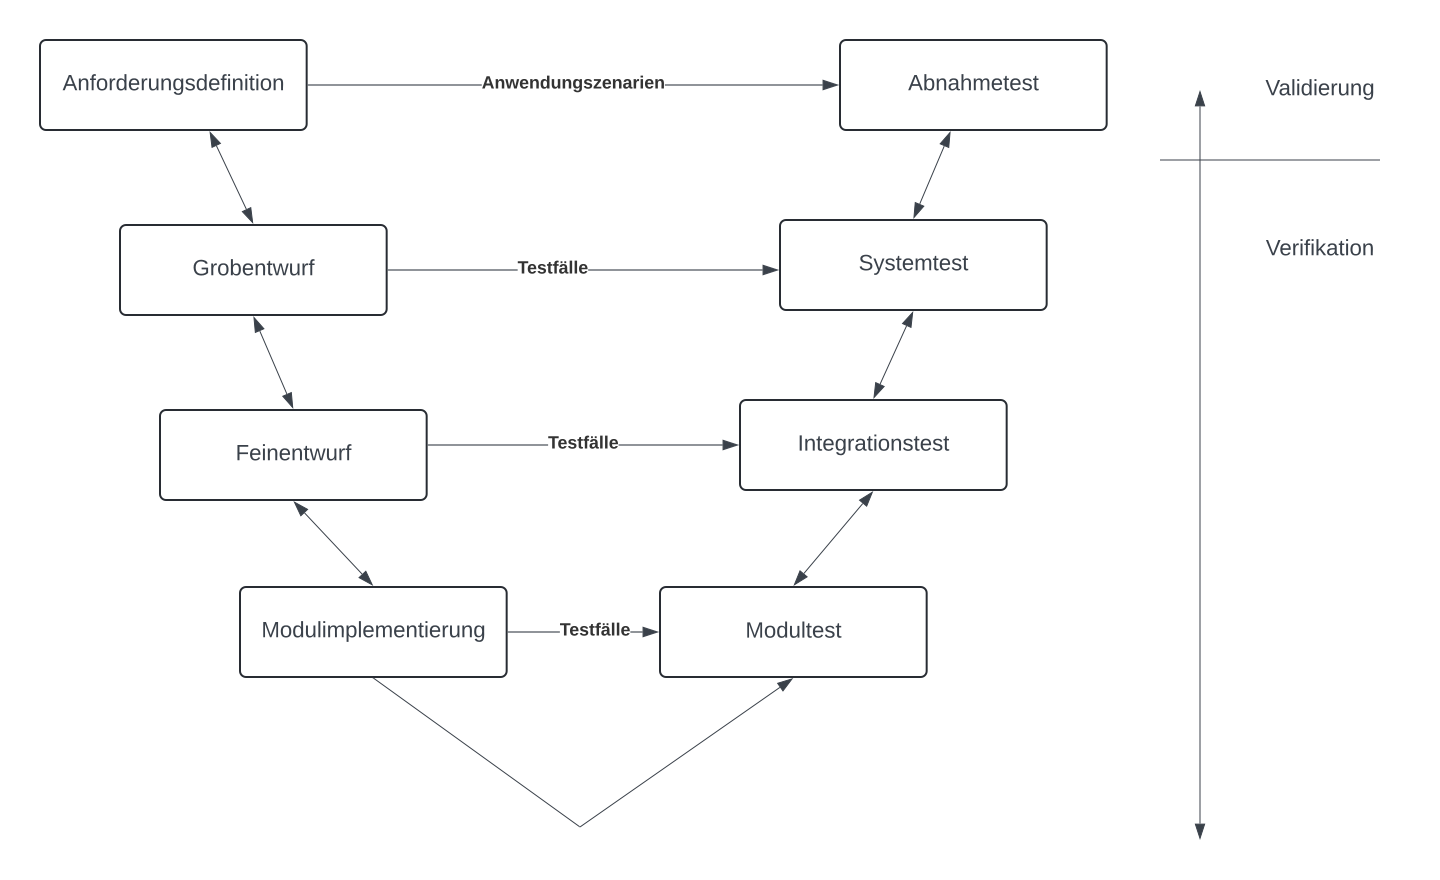
\includegraphics[scale=0.3]{chapters/Glossar/img/vmodell}
    \caption{Das Vorgehensmodell nach Boehm. (Quelle: in Anlehnung an \cite[554, Abb. 20.11-2]{Bal08})}
    \label{fig:v-modell-cc}
\end{figure}
